\documentclass{tufte-handout}
\usepackage{amsmath,amsthm}

\usepackage{pgfplots}
%\pgfplotsset{width=\textwidth,compat=1.5.1}

\newtheorem{claim}{Claim}[section]
\title{\sf Rainbow Perfect Matchings}
\author{Mats Rydberg \& Martin Larsson}

\begin{document}
\maketitle

\begin{marginfigure}
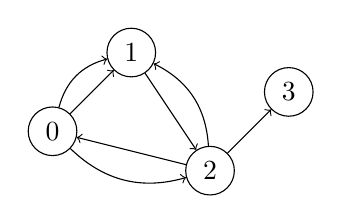
\begin{tikzpicture}
\node (0) [draw,circle] at (0,0) {0};
\node (1) [draw,circle] at (1,1) {1};
\node (2) [draw,circle] at (2,-.5) {2};
\node (3) [draw,circle] at (3,.5) {3};
\draw [->] (0) to [bend left] (1);
\draw [->] (0) to  (1);
\draw [->] (0) to [bend right] (2);
\draw [->] (1) to  (2);
\draw [->] (2) to  (0);
\draw [->] (2) to [bend right] (1);
\draw [->] (2) to (3);
\end{tikzpicture}
\caption{A directed multigraph.}
\end{marginfigure}

\section{Algorithm}

\section{Analysis}

\subsection{Lol}

The files are in the data directory are:
\begin{quotation}
\begin{description}
\item[three.txt] The 4-vertex graph from Fig.~1.
\end{description}
\end{quotation}

\section{Report part maybe}

\subsection{Transition probabilities}

The transition matrix for the graph described in three.txt
is\sidenote{Fill in the right values. Set $\alpha=\frac{85}{100}$.}
\begin{equation*}
P = 
\left(
\begin{array}{cccc}
1 & 6 & \pi & 1\\
1 & 1/e & -2  & \cdots\\
1 & 1 & 0 \\
\vdots
\end{array}
\right)\,,
\end{equation*}

\noindent text is text is text is text

\medskip
\begin{fullwidth}
\small
\begin{tabular}{lcccccccccc}
three.txt & 2 (36.6\%) & 1 (27.5\%) & 0 (18.4\%) & 3 (17.3\%) \\
tiny.txt & [\ldots] &\\
medium.txt &\\
wikipedia.txt & \\
p2p-Gnutella08-mod.txt &
\end{tabular}
\end{fullwidth}

\end{document}
